\section{Kết quả so sánh các mô hình truyền thống}
\label{sec:6_1}
Các bảng trong mục 6.1--6.4 là kết quả CV trên train, chưa phải kết quả test. Chọn cấu hình tốt nhất của mỗi họ trong phạm vi scope=model với tiền xử lý cơ sở. F1, precision và recall đều tính cho lớp \texttt{>50K}.
\begin{table}[htbp]
\centering\scriptsize
\caption{Kết quả CV của các mô hình truyền thống và mốc đa số}\label{tab:cv-traditional}
\begin{tabular}{lrrrr}
\toprule
Cấu hình & F1 CV & SD & Precision & Recall \\
\midrule
dummy\_majority & 0,0000 & 0,0000 & 0,0000 & 0,0000 \\
svm\_c1 & 0,6514 & 0,0028 & 0,7375 & 0,5833 \\
lr\_c1 & 0,6557 & 0,0078 & 0,7315 & 0,5943 \\
rf\_full\_leaf3 & 0,6782 & 0,0012 & 0,7756 & 0,6026 \\
\bottomrule
\end{tabular}
\end{table}
\begin{figure}[htbp]
\centering
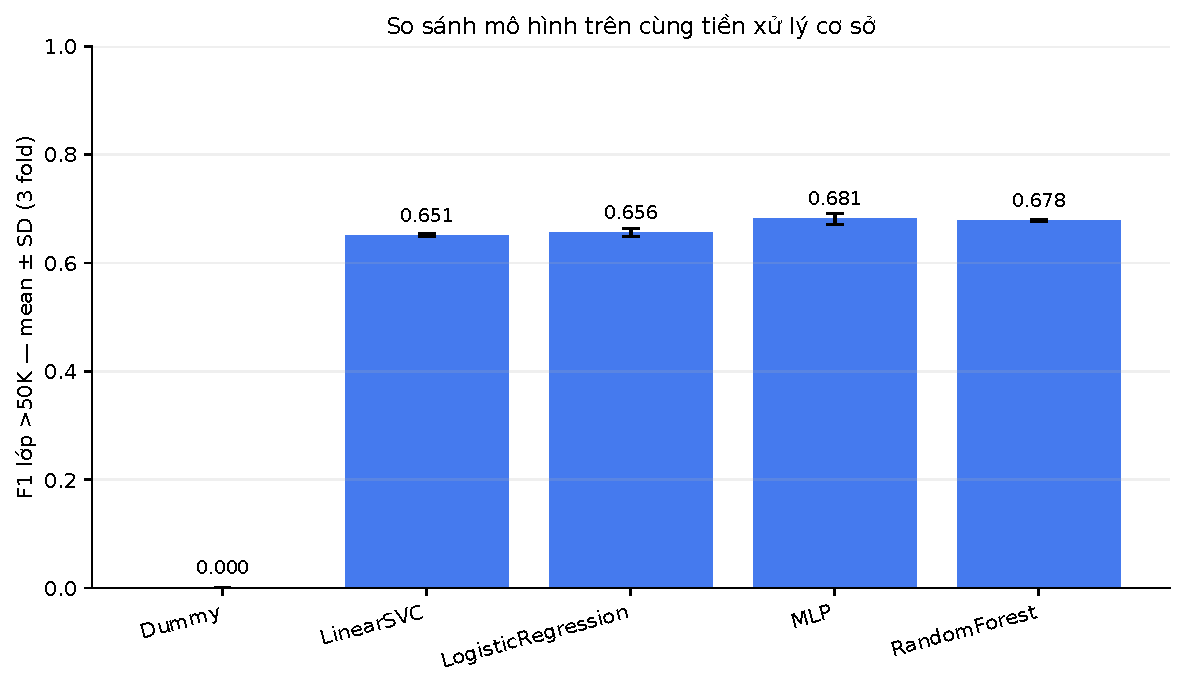
\includegraphics[width=.95\textwidth]{Images/chapter_6/6_1/cv_models.pdf}
\caption{F1 CV của cấu hình tốt nhất mỗi họ trên tiền xử lý cơ sở; thanh sai số là SD qua ba fold}
\label{fig:cv-models}
\end{figure}
Mốc đa số có F1 lớp dương bằng 0 dù accuracy có thể cao, cho thấy chỉ dùng accuracy là chưa đủ. Các họ mô hình học từ thuộc tính cần được đánh giá cùng precision và recall để thấy mức đánh đổi khi phát hiện nhóm thu nhập cao.

% BEGIN REVIEW ANALYSIS
Trong nhóm mô hình truyền thống, Random Forest có F1 CV cao nhất là 0,6782, hơn Logistic Regression cơ sở 2,25 điểm phần trăm và hơn LinearSVC 2,69 điểm phần trăm. Đây là đối chứng truyền thống chính của bài làm; pipeline đã được ghép tiền xử lý, huấn luyện và đánh giá bằng CV cùng validation. Số cấu hình tìm kiếm giữa các họ không bằng nhau nên bảng so sánh phản ánh thiết kế cụ thể đã chạy.
% END REVIEW ANALYSIS
